


\chapter{Grundlagen}

\section{Appstudio}
SICK AppSpace - Engineering-Framework für Ihre individuellen Sensoranwendungen

SICK AppSpace ist ein Ökosystem rund um programmierbare Sensoren und Geräte von SICK und individualisierte SensorApps. Als Teil einer dynamischen Entwickler-Community können Kunden eigenständig oder gemeinsam mit den Experten von SICK SensorApps erstellen. Mit diesen SensorApps lassen sich alle Anwendungen mit unterschiedlichsten Technologien lösen. Individualisierte SensorApps werden mit intelligenten Softwaretools und Algorithmen erstellt. Bestehende Lösungen für Track & Trace, Positionieraufgaben, Roboterführung oder Qualitätskontrolle können an die individuellen Bedürfnisse der Kunden angepasst werden; und völlig neue SensorApps können nach individuellen Anforderungen und absolut maßgeschneidert für bestehende Systeme erstellt werden. SICK AppSpace unterstützt heute eine Reihe von Geräten und Technologien, wie 2D-Vision, 3D-Vision, LiDAR, RFID oder Integrationsprodukte. Das SICK-AppSpace-Ökosystem besteht aus drei Hauptkomponenten. Zum einen aus der Hardware, das heißt programmierbare Sensoren, Sensorintegrationsmaschinen und andere Geräte. Zum anderen Software und Tools, das heißt die Werkzeuge zum Erstellen, Verteilen und Bereitstellen von SensorApps. Und als letzten Hauptkomponenten die Community, das heißt die Mitglieder des SICK AppSpace-Entwicklerclubs, die sich im SICK Support Portal und Konferenzen austauschen.

Die programmierbaren Geräte im SICK-AppSpace-Ökosystem bieten Raum für die Integration der kundenspezifischen SensorApps und ermöglichen so maßgeschneiderte Applikationslösungen. So werden je nach Anwendung völlig neue Lösungen im Bereich der Automatisierung möglich - und die SensorApps können jederzeit angepasst oder ausgetauscht werden. SICK AppSpace-Sensoren und -Geräte bieten eine "Dual Talk"-Funktion, die eine gleichzeitige Kommunikation mit einer SPS sowie mit übergeordneten Enterprise-Level-Systemen und sogar Cloud-Services ermöglicht. Sie unterstützen damit den Aspekt der vertikalen Integration von Industrie 4.0.

Das AppEngine-Framework ist das Herzstück der Firmware bei allen programmierbaren Geräten. Es bietet eine umfangreiche Anwendungsprogrammierschnittstelle (SICK Algorithm API) mit einem breiten, gerätespezifischen Satz an vordefinierten Funktionen und Operatoren. Geräte mit Bildverarbeitung bieten zwei Methoden der Bildverarbeitung - entweder mit den 2D- und 3D-Operatoren der SICK Algorithm API oder mit der integrierten leistungsfähigen HALCON-Vision-Bibliothek.

Die zentralen Werkzeuge im SICK AppSpace-Ökosystem sind das SICK AppStudio, der SICK AppManager und der SICK AppPool.


Das SICK AppStudio ist eine integrierte Anwendungsentwicklungsumgebung zur Erstellung von SensorApps. Mit diesen SensorApps können Entwickler kundenspezifische Applikationslösungen auf programmierbaren Geräten erstellen. SensorApps können mit Standardkomponenten und Programmiersprachen programmiert werden. Anwendungsentwickler mit weniger Interesse am Programmieren können auch Datenflüsse modellieren, wobei ein tieferes Eintauchen in die Programmierung immer möglich ist. Die Benutzeroberflächen der SensorApps sind webbasiert, so dass sie in jedem Browser angezeigt werden können. Sie können vom SensorApp-Entwickler über einen grafischen UI-Builder oder mit Standard-Webtechnologien individuell gestaltet werden.

 

SensorApps werden mit dem Deployment-Tool SICK AppManager installiert, aktualisiert und verwaltet. Es integriert sich direkt in den SICK AppPool und unterstützt das automatische Deployment über ein CLI. Der vollständige SICK AppManager ist kostenlos und für Windows (x64) verfügbar, die reine CLI-Version ist auch für Windows-32bit-, Linux-64bit- und ARM-32bit-Systeme verfügbar.

 

Der SICK AppPool ist der zentrale und sichere Cloud-Service zum Austausch von SensorApps. SensorApp-Entwickler können ihre SensorApps veröffentlichen und entweder mit einer ausgewählten Gruppe von Nutzern oder mit der ganzen Welt teilen. Interessierte können SensorApps nach Stichworten, kompatiblen Geräten, Applikationen, Herausgebern und zahlreichen weiteren Filtern finden. Die Veröffentlichung im SICK AppPool ist ein Privileg der Mitglieder des SICK AppSpace Developers Club.

 

Um SensorApps zu entwickeln, ist eine Mitgliedschaft im SICK AppSpace Developers Club erforderlich. Diese Mitgliedschaft beinhaltet eine Volllizenz für das SICK AppStudio. Für die Dauer von einem Jahr haben Mitglieder außerdem Zugriff auf das Ticket-Supportsystem im SICK Support Portal, Entwicklerschulungen, exklusive Downloads und viele weitere Vorteile. Darüber hinaus werden sie zu den jährlichen SICK AppSpace-Entwicklerkonferenzen und anderen Veranstaltungen eingeladen, wo sie ihre Arbeit präsentieren, Ideen austauschen und die Entwicklung des SICK AppSpace-Ökosystems mitgestalten können.

\section{LUA}

Lua ist eine imperative und erweiterbare Skriptsprache zum Einbinden in Programme, um diese leichter weiterentwickeln und warten zu können. Eine der besonderen Eigenschaften von Lua ist die geringe Größe des kompilierten Skript-Interpreters.

Lua-Programme sind meist plattformunabhängig und werden vor der Ausführung in Bytecode übersetzt. Obwohl man mit Lua auch eigenständige Programme schreiben kann, ist sie vorrangig als eingebettete Skriptsprache für andere Programme konzipiert. Vorteile von Lua sind die geringe Größe von 120 kB, die Erweiterbarkeit und die hohe Geschwindigkeit, verglichen mit anderen Skriptsprachen.

Der Lua-Interpreter kann über eine C-Bibliothek angesprochen werden, die auch ein API\footnote{von englisch application programming interface, wörtlich ‚Anwendungs­programmier­schnittstelle} für die Laufzeitumgebung des Interpreters für Aufrufe vom C-Programm aus enthält. Mittels des API können verschiedene Teile des Programmes in C (oder C++) und Lua geschrieben werden, während Variablen und Funktionen in beiden Richtungen erreichbar bleiben (d. h. eine Funktion in Lua kann eine Funktion in C/C++ aufrufen und umgekehrt).

\subsection{Ausführung von Lua-Dateien}

Durch die Dokumentation wurden Erfahrungen mit Lua gesammelt.\cite{Ierusalimschy.2006} Um Code zu testen, wird dieser mit dem Editor oder mit Visual Studio geschrieben. Der Ordner, in der die geschriebene Lua-Datei liegt, wird im Explorer geöffnet. Anstelle des Datei-Pfades wird CMD eingegeben. Das CMD Fenster öffnet sich, dort wird der Befehl lua54 "Name der Lua-Datei".lua und die Datei wird ausgeführt. Der Output lässt sich im CMD finden.\cite{Ierusalimschy.2013}

\section{LMS4000}

\begin{figure}[h]
\centering
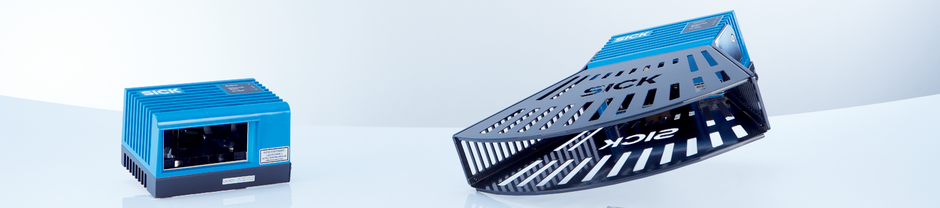
\includegraphics[width=13cm]{Bilder/LMS4000.png}
\caption{LMS4000 mit und ohne Strahlenschutz}
\label{LMS4000 mit und ohne Strahlenschutz}
\end{figure}



Der 2D-LiDAR-Sensor LMS4000 ist besonders geeignet für den Einsatz in Intralogistik, Materialhandling und allen Bereichen, in denen Güter schnell und zielgenau analysiert und bewegt werden müssen. Mit dem LMS4000 bietet SICK die ideale Lösung, um Objekte hinsichtlich ihrer Lage, Form, Volumen oder Oberflächenbeschaffenheit zu vermessen und sie dementsprechend zu bewerten und weiterzuverarbeiten. Unabhängig von der Objektposition in Behältern, Kartons, auf Paletten, freistehend oder einander berührend, misst der Sensor präzise mit hoher Abtastdichte und weitem Dynamikbereich. Ein hoher Durchsatz bei gleichzeitig umfassender Prozesssicherheit und geringem Wartungsaufwand sind das Ergebnis.

Der 2D-LiDAR-Sensor LMS4000 liefert als Einzelkomponente in der automatisierten Fertigung exakte Daten über Position und Größe unterschiedlichster Objekte. Der Sensor gibt diese Daten, häufig in Verbindung mit einem Encoder, an eine externe Auswerteeinheit weiter. Hieraus ergeben sich unterschiedlichste Einsatzbereiche, wie beispielsweise bei der Volumen- und Lagebestimmung von Objekten, Pick & Place bzw. Palettierungs- und Depalettierungsaufgaben, Leerbehälterkontrolle, Qualitätsinspektion von Solarzellen über Motorblöcke bis hin zu Flugzeugteilen, Zügen oder Tunnelwänden und vieles mehr.

\subsection{Objektvermessung}

Der LMS4000 vermisst Objekte unabhängig von ihrer Form, Farbe oder Oberflächenbeschaffenheit. Mit einem Öffnungswinkel von 70° entsteht ein breiter Scanbereich, den ein kontinuierlicher Laser über den rotierenden Sechskantspiegel mit 600 Hz abtastet. Jeder Scan generiert dabei 841 Einzelmesspunkte. Die Verwendung eines Rotlichtlasers im sichtbaren Spektrum erleichtert die exakte Ausrichtung.

Objekte mit einer Höhe von 1 m werden mit dem LMS4000 durchgängig auf einer Breite von 2,6 m vermessen. Bei 2 m hohen Objekten kann die Messfeldbreite bis zu 1,4 m betragen. Die Gerätevariante mit erhöhter Reichweite ermöglicht darüber hinaus sogar das Vermessen von Objekten mit einem Querschnitt von 3 m x 3 m oder auch 4 m x 2 m.

Der Laserscanner lässt sich gezielt über Lichtschranken oder Softwarebefehle ein- und ausschalten. So fallen nur dann Daten an, wenn tatsächlich ein Objekt vermessen wird. Interne Filter erlauben die zielgerichtete Reduktion von Daten auf die spezifische Applikation und entlasten dadurch zusätzlich das Gesamtsystem.

Das Continuous-Wave-Verfahren basiert auf dem Prinzip der Phasenkorrelation. Das Objekt reflektiert dabei den kontinuierlich ausgesendeten Laserstrahl auf den Empfänger des Laserscanners. Aus dem resultierenden Phasenlaufzeitunterschied zwischen Sende- und Empfangsstrahl lässt sich präzise die Distanz ermitteln. Gleichzeitig ist das Messverfahren widerstandsfähig gegen externe Beeinflussung, z. B. durch Fremdlicht oder Temperaturschwankungen.

Neben Distanzdaten übermittelt der Sensor bei Bedarf auch Remissions-, Winkelkorrektur- und Gütewerte. Dadurch können bereits geringe Unterschiede in Farbe und Textur von Objekten sichtbar gemacht, auf den Sensor einwirkende Beschleunigungen kompensiert, sowie kritische Messpunkte identifiziert werden. Das Ausgabedatenformat kann dabei individuell um jeden Kanal erweitert oder reduziert werden.

Der Einsatz mehrerer Laserscanner verhindert Abschattungseffekte und ermöglicht größere Messfelder. Die Motoren der rotierenden Spiegel lassen sich über das System miteinander synchronisieren, sodass sich die Geräte nicht gegenseitig beeinflussen.\cite{.31.08.2022}

\section{Encoder}
Im vorliegenden Demokoffer wird der Inkremental-Encoder DBS36/50 verwendet. Inkremental-Encoder erzeugen Informationen über Lage, Winkel und Umdrehungszahlen. Die Auflösung wird in Anzahl der Striche bzw. Impulse pro Umdrehung definiert, welche der Encoder für jede Umdrehung an die Steuerung weitergibt. Die aktuelle Position kann von der Steuerung durch das Zählen dieser Impulse ermittelt werden. Beim Einschalten der Maschine kann eine Referenzfahrt notwendig werden.\cite{.31.08.2022b}
Inkremental-Encoder DBS36/50 zeichnen sich durch hohe mechanische Flexibilität, herausragende technische Eigenschaften und
viele Variantenaus. Die Encoder sind mit Gehäusedurchmessern von 36 mm und 50 mm sowie mit verschiedenen Aufsteckhohl-
wellen und Vollwellen erhältlich. Durch unterschiedliche Montagelochbilder, Servoklammern und Servonuten und universelle Dreh-
momentstützen bieten DBS36/50 umfangreiche Montagemöglichkeiten. Alle Modelle haben kompakte Abmessungen und einen
universellen Leitungsanschluss. Dieser ermöglicht sowohl axiale als auch radiale Leitungsführung. Der DBS36/50 hat 2.500 Impulse pro Umdrehung. Die Kommunikationsschnittstellen TTL/RS-422, HTL/Push pull und Open Collector. Die Anschlussart ist eine Leitung mit Stecker M12 und M23.



\section{Clean Coding}


